%
% kont.tex
%
% (c) 2025 Prof Dr Andreas Müller
%
\documentclass[tikz]{standalone}
\usepackage{times}
\usepackage{amsmath}
\usepackage{txfonts}
\usepackage[utf8]{inputenc}
\usepackage{graphics}
\usetikzlibrary{arrows,intersections,math}
\usepackage{ifthen}
\begin{document}

\newboolean{showgrid}
\setboolean{showgrid}{false}
\def\breite{6}
\def\hoehe{5}

\definecolor{blau}{rgb}{0.2,0.6,1.0}

\begin{tikzpicture}[>=latex,thick]

% Povray Bild
\node at (0,0) {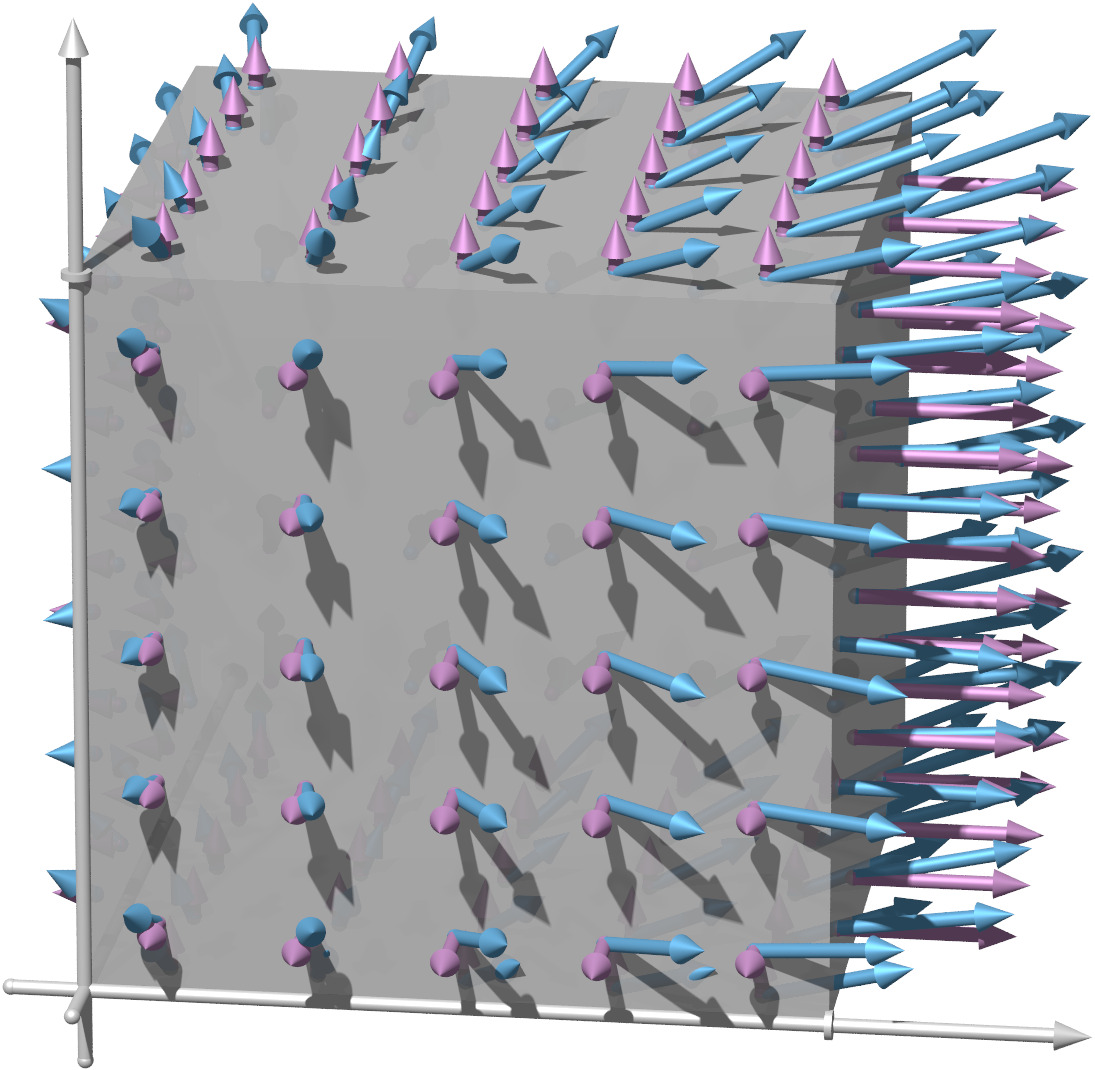
\includegraphics[width=10.0cm]{kont.jpg}};

% Gitter
\ifthenelse{\boolean{showgrid}}{
\draw[step=0.1,line width=0.1pt] (-\breite,-\hoehe) grid (\breite, \hoehe);
\draw[step=0.5,line width=0.4pt] (-\breite,-\hoehe) grid (\breite, \hoehe);
\draw                            (-\breite,-\hoehe) grid (\breite, \hoehe);
\fill (0,0) circle[radius=0.05];
}{}

\node at (2.56,-4.75) {$\Delta x$};
\node at (-4.69,2.4) {$\Delta z$};
\node at (-3.45,4.4) {$\Delta y$};

\node at (5.05,-4.4) {$x$};
\node at (-4.55,4.7) {$z$};

\node[color=blau] at (4.8,4.1) {$\vec{v}(x,y,z)$};

\end{tikzpicture}

\end{document}

